\section{Results}
\label{sec:results}

% Evidence: research_os/paper/canonical/data.json; macros.tex; tables/*.tex;
% latex/figures (from paper/figures / experiments/results); paper/analysis.md; paper/conclusion.md.
% Results report observed outcomes only (What happened?). Mechanism deferred to Discussion.

All headline test-error values and signed deltas below are taken from the paper canonical
snapshot via macros (Section~\ref{sec:setup}).
Unless noted, each completed model is a \emph{single} training run with unset seed.

\subsection{Main Results}
\label{sec:results-main}

Table~\ref{tab:main-results} lists best test error, best epoch, parameter count, and run status
for Plain-20, ResNet-20-A, PreAct-ResNet-20-A, Ablation~A, and Ablation~B.
Table~\ref{tab:deltas} reports the corresponding pairwise differences in best test error
(percentage points).

\begin{table}[t]
  \caption{Main CIFAR-10 results (best test error). Numbers are from the canonical snapshot.
  Ablation~B has no comparable best test error.}
  \label{tab:main-results}
  \centering
  \small
  % AUTO-GENERATED — do not edit by hand
% Source: research_os/paper/canonical/data.json
\begin{tabular}{lrrrl}
\toprule
Model & Best test err. (\%) & Best epoch & Params & Status \\
\midrule
  Plain-20 & 9.68 & 132 & 270,410 & completed \\
  ResNet-20-A & 8.41 & 132 & 270,410 & completed \\
  PreAct-ResNet-20-A & 9.47 & 128 & 270,314 & completed \\
  Ablation-A & 8.32 & 124 & 269,738 & completed \\
  Ablation-B & N/A & --- & 269,642 & failed (numerical\_instability) \\
\bottomrule
\end{tabular}

\end{table}

\begin{table}[t]
  \caption{Pairwise differences in best test error (percentage points; canonical deltas).}
  \label{tab:deltas}
  \centering
  \small
  % AUTO-GENERATED — do not edit by hand
\begin{tabular}{lr}
\toprule
Comparison & $\Delta$ best test err. (pp) \\
\midrule
ResNet-20-A $-$ Plain-20 & -1.27 \\
PreAct $-$ ResNet-20-A & 1.06 \\
Ablation-A $-$ ResNet-20-A & -0.09 \\
Ablation-A $-$ PreAct & -1.15 \\
\bottomrule
\end{tabular}

\end{table}

Observed best test errors for completed runs:
Plain-20 $\ErrPlain\%$;
ResNet-20-A $\ErrResNet\%$;
PreAct-ResNet-20-A $\ErrPreAct\%$;
Ablation~A $\ErrAblationA\%$.
Ablation~B did not complete as a comparable accuracy run
(status \AblationBStatus).

Figure~\ref{fig:phase4-bar} summarizes best test error for the Phase~4 triad
(Plain-20 / ResNet-20-A / PreAct-ResNet-20-A).
Figure~\ref{fig:phase5-bar} includes completed Phase~5 models together with the frozen baselines.

\begin{figure}[t]
  \centering
  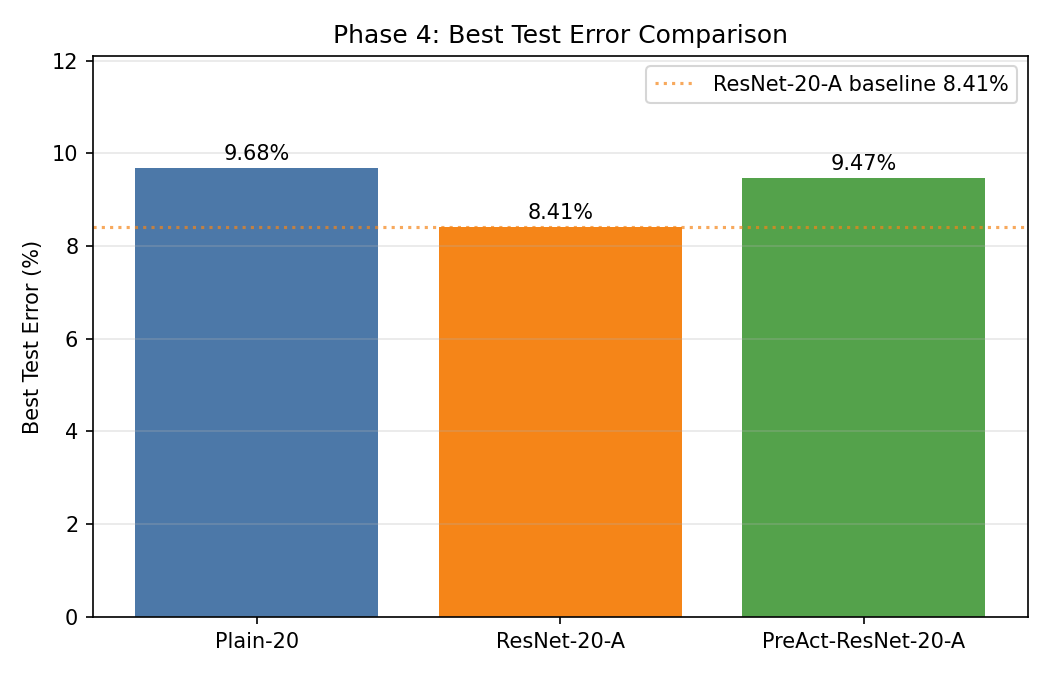
\includegraphics[width=0.82\linewidth]{phase4_best_test_error_bar.png}
  \caption{Best test error for Plain-20, ResNet-20-A, and PreAct-ResNet-20-A
  (Phase~4 comparison figure).}
  \label{fig:phase4-bar}
\end{figure}

\begin{figure}[t]
  \centering
  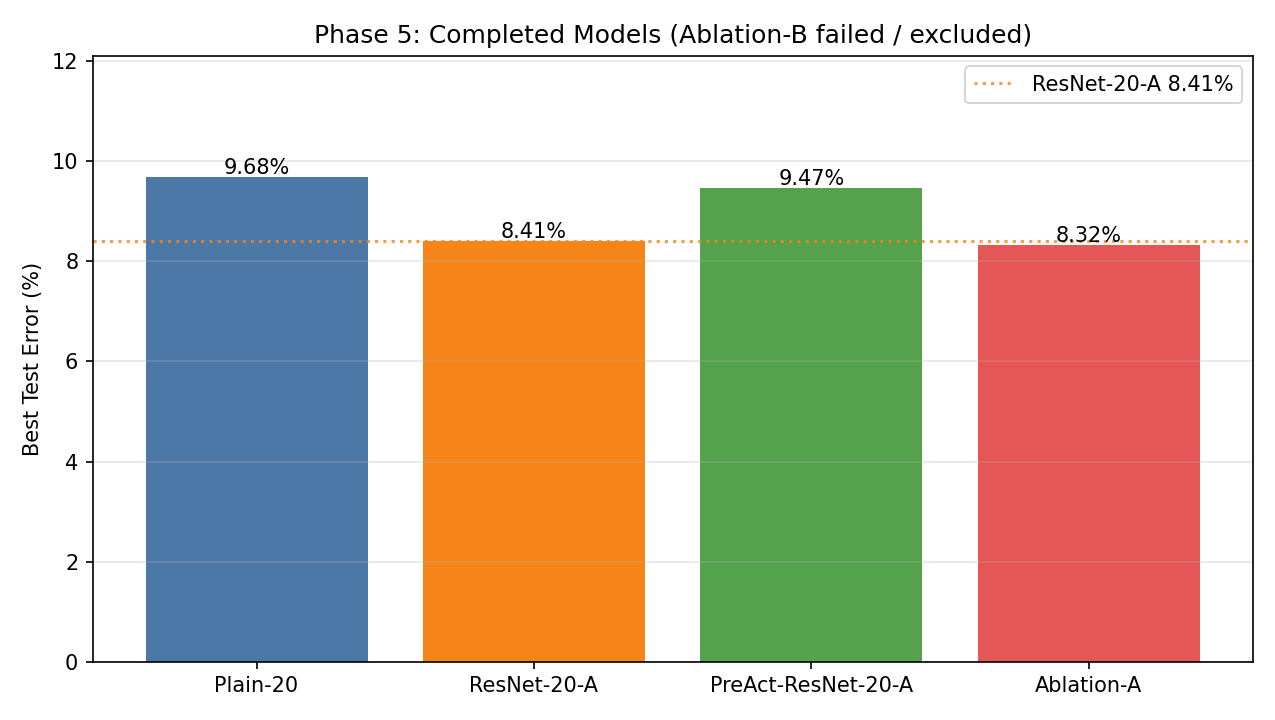
\includegraphics[width=0.82\linewidth]{phase5_best_test_error.png}
  \caption{Best test error among completed models in the Phase~5 summary figure
  (Ablation~B omitted as a failed run).}
  \label{fig:phase5-bar}
\end{figure}

\subsection{Residual Learning Comparison}
\label{sec:results-residual}

Under the shared protocol, ResNet-20-A attains best test error $\ErrResNet\%$,
while Plain-20 attains $\ErrPlain\%$.
The residual model is lower by $\ResidualAdvantagePP$ percentage points
(equivalently, ResNet-20-A $-$ Plain-20 $= \DeltaResNetMinusPlain$\,pp;
Table~\ref{tab:deltas}).

Relative to the He et~al.\ CIFAR ResNet-20 reference value $\PaperResNetRef\%$
(Table~6 in the source paper; stored as a canonical reference scalar, not a run of this project),
the observed ResNet-20-A error differs by less than the preset absolute tolerance
$\ReproTolerancePP$\,pp used in the reproduction notes
(status \ReproStatus; depth-20 subset only).

Figure~\ref{fig:phase2-plain-vs-res} shows the Phase~2 plain-vs-residual comparison plot
associated with these two completed baseline runs.

\begin{figure}[t]
  \centering
  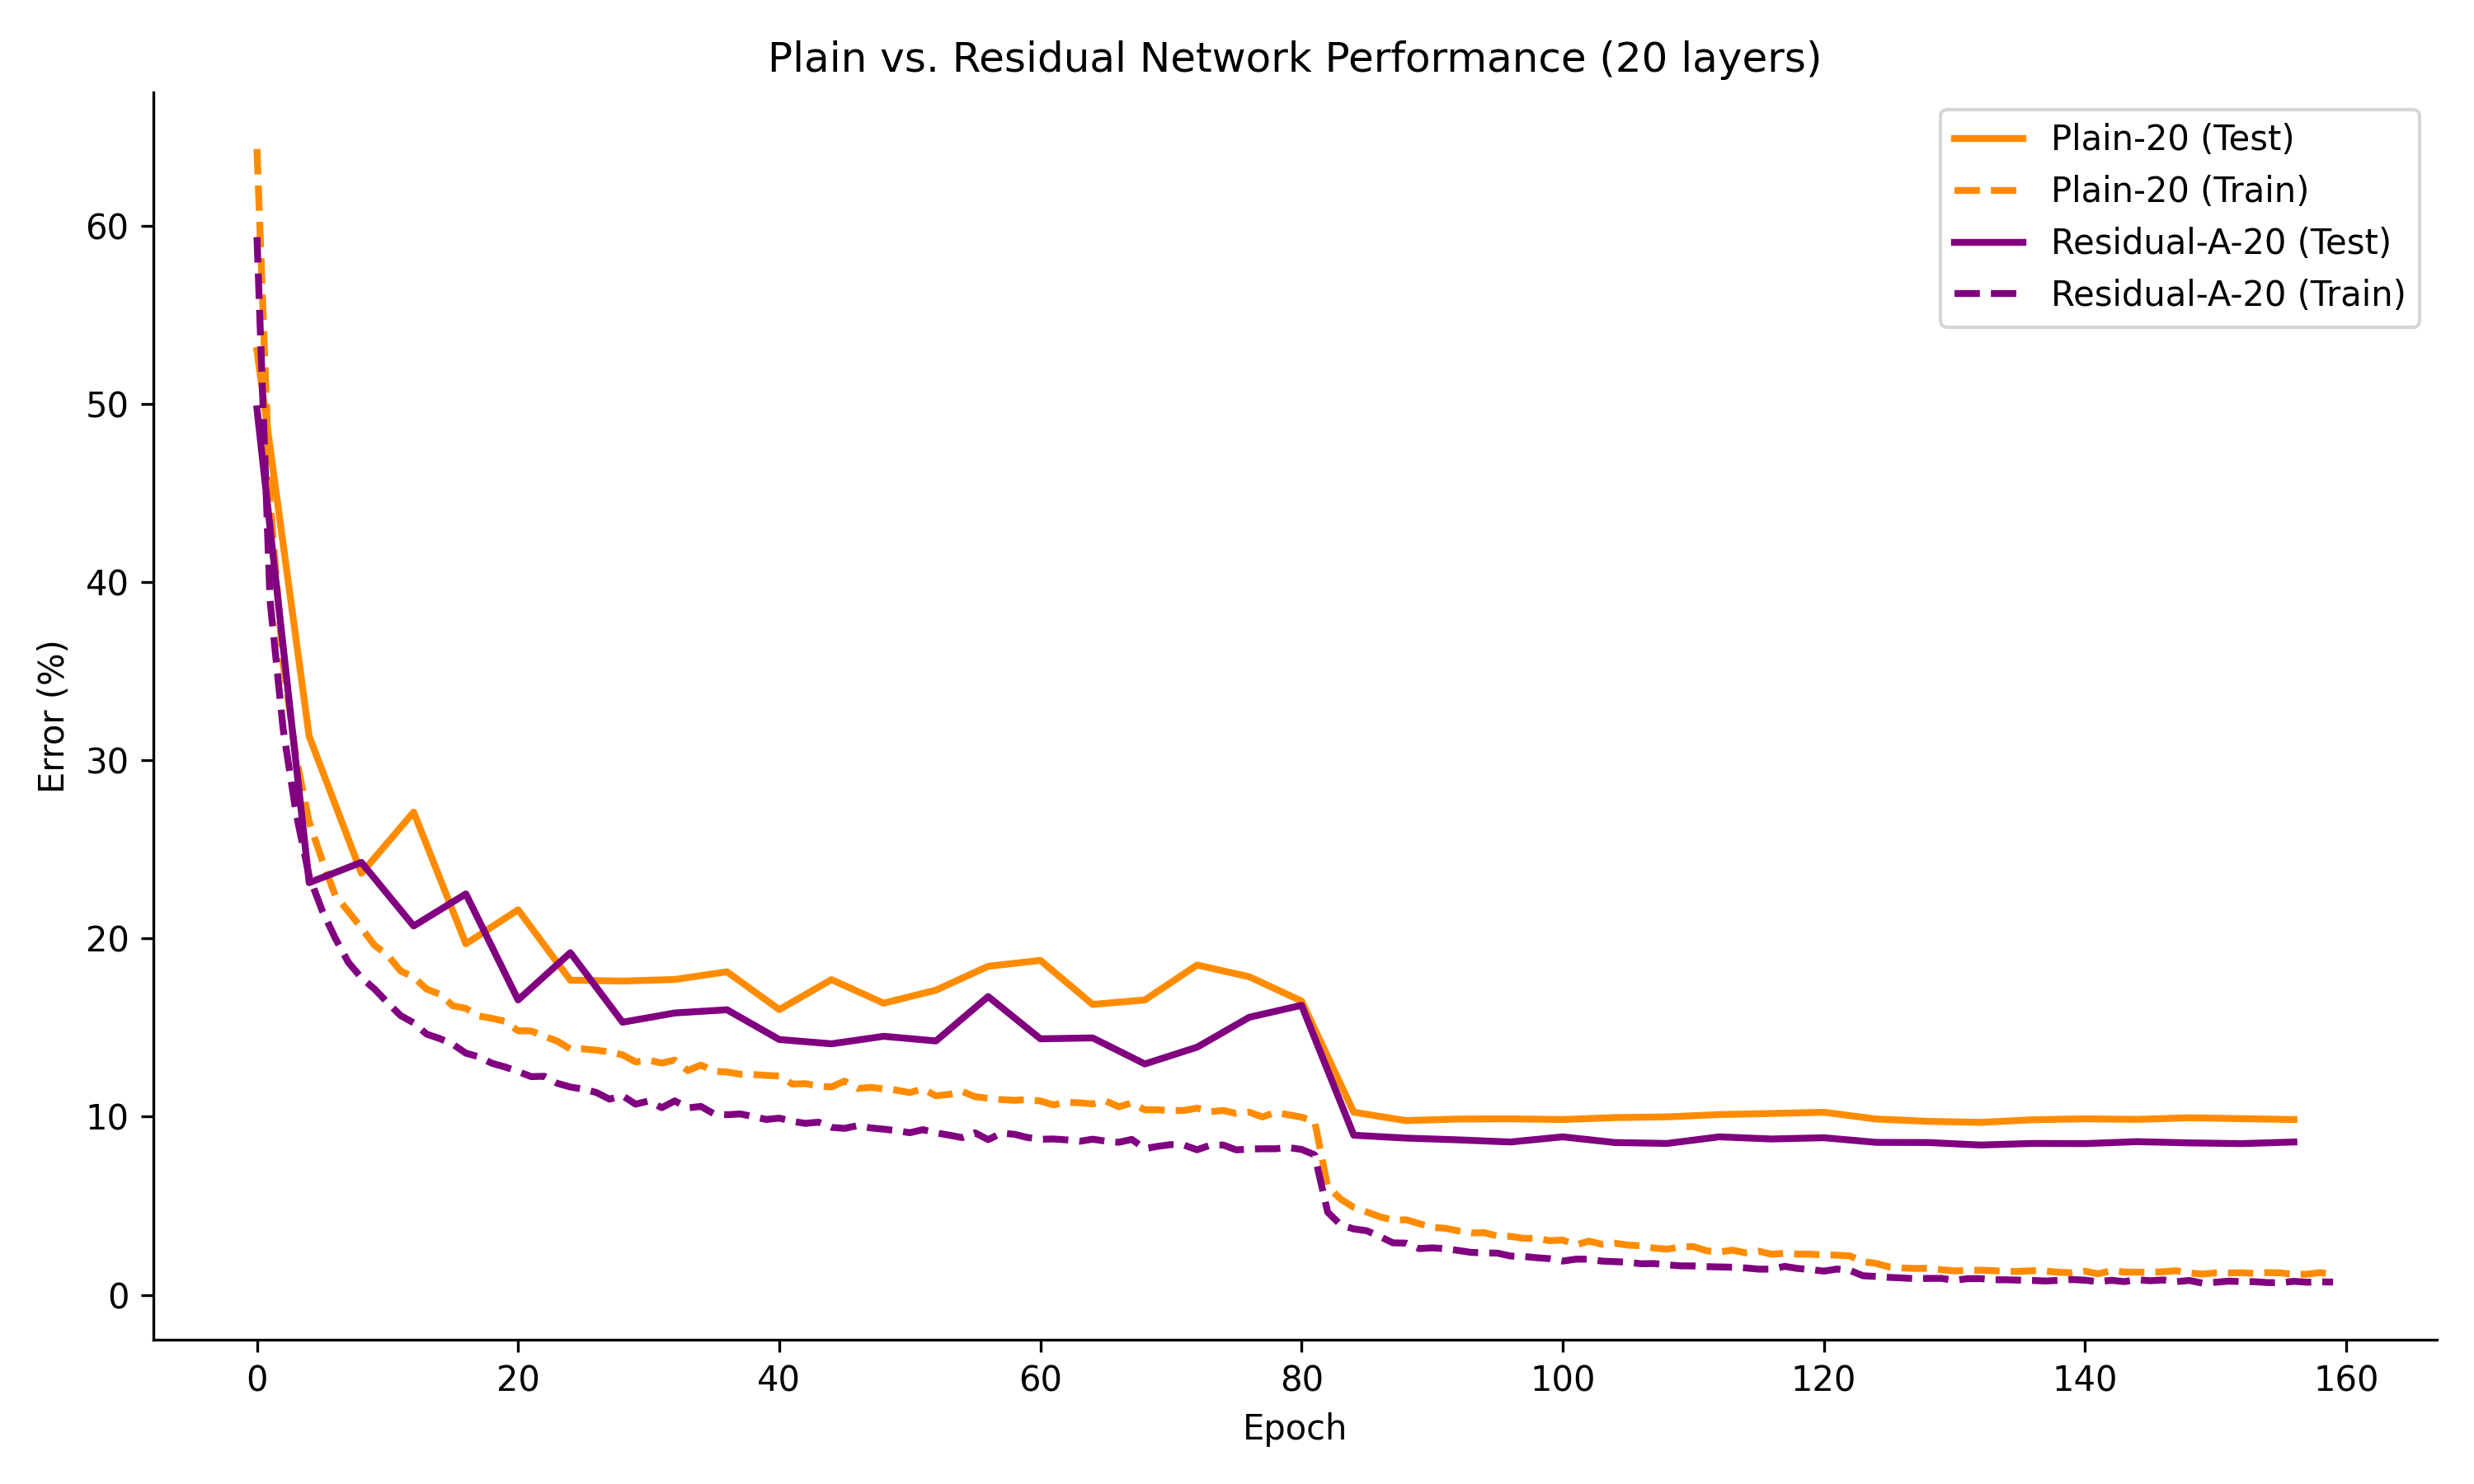
\includegraphics[width=0.82\linewidth]{phase2_plain_vs_residual.png}
  \caption{Phase~2 plain vs.\ residual comparison figure for the frozen depth-20 pair.}
  \label{fig:phase2-plain-vs-res}
\end{figure}

\subsection{Pre-activation Improvement}
\label{sec:results-preact}

With dataset, Option~A, depth, and the frozen post-activation training recipe held fixed,
replacing the residual block by the full pre-activation unit yields
PreAct-ResNet-20-A best test error $\ErrPreAct\%$.
Relative to ResNet-20-A ($\ErrResNet\%$), this is an increase of
$\DeltaPreActMinusResNet$ percentage points
(PreAct $-$ ResNet-20-A $= \DeltaPreActMinusResNet$\,pp; Table~\ref{tab:deltas}).

Thus, under this single-run frozen-recipe comparison, the pre-activation substitution
does \emph{not} reduce test error relative to the frozen ResNet-20-A control.
Figure~\ref{fig:phase4-curves} shows the corresponding Phase~4 test-error curves.

\begin{figure}[t]
  \centering
  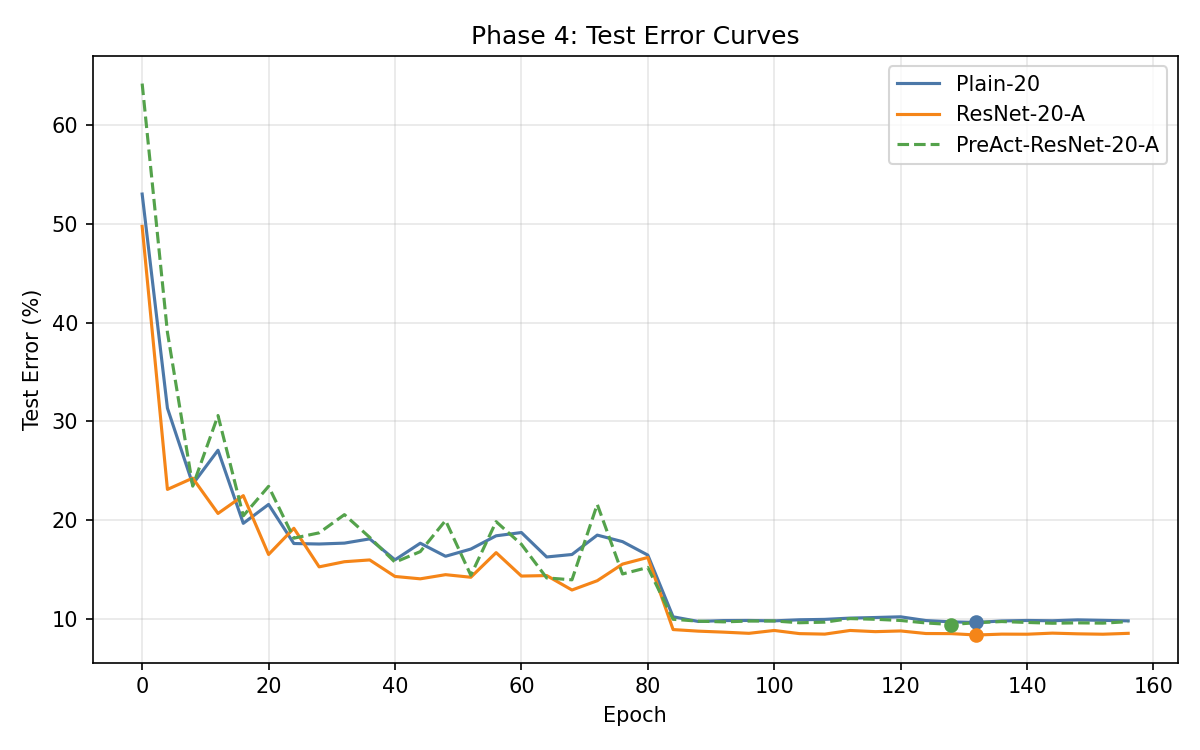
\includegraphics[width=0.82\linewidth]{phase4_test_error_curves.png}
  \caption{Phase~4 test-error curves for Plain-20, ResNet-20-A, and PreAct-ResNet-20-A.}
  \label{fig:phase4-curves}
\end{figure}

\subsection{Ablation Results}
\label{sec:results-ablation}

\paragraph{Ablation~A.}
Removing the first $\mathrm{BN}{+}\mathrm{ReLU}$ from the full PreAct unit yields
best test error $\ErrAblationA\%$.
Versus full PreAct ($\ErrPreAct\%$), Ablation~A is lower by
$\DeltaAblationAVsPreAct$ percentage points in magnitude
(Ablation~A $-$ PreAct $= \DeltaAblationAMinusPreAct$\,pp).
Versus ResNet-20-A ($\ErrResNet\%$), Ablation~A differs by
$\DeltaAblationAMinusResNet$ percentage points
(Ablation~A $-$ ResNet-20-A $= \DeltaAblationAMinusResNet$\,pp).
This latter gap is a small single-run difference and is reported as an observed delta only.

\paragraph{Ablation~B.}
Removing the second $\mathrm{BN}{+}\mathrm{ReLU}$ produced a failed training run with
numerical instability (status \AblationBStatus).
No best test error is reported for Ablation~B, and the failed trajectory is \emph{not}
used as an accuracy baseline in Table~\ref{tab:main-results} or Table~\ref{tab:deltas}.

\subsection{Summary of Observations}
\label{sec:results-summary}

Under the frozen CIFAR-10 depth-20 protocol of Section~\ref{sec:setup}, the recorded outcomes are:
\begin{enumerate}
  \item ResNet-20-A ($\ErrResNet\%$) improves on Plain-20 ($\ErrPlain\%$) by
        $\ResidualAdvantagePP$\,pp.
  \item Full PreAct-ResNet-20-A ($\ErrPreAct\%$) has higher best test error than ResNet-20-A by
        $\DeltaPreActMinusResNet$\,pp on this single run.
  \item Ablation~A ($\ErrAblationA\%$) is better than full PreAct by
        $\DeltaAblationAVsPreAct$\,pp in magnitude, and differs from ResNet-20-A by
        $\DeltaAblationAMinusResNet$\,pp.
  \item Ablation~B fails with numerical instability and contributes no comparable
        best-test-error number.
\end{enumerate}
Interpretation of mechanisms and broader generalization is deferred to the discussion.
